\documentclass[aspectratio=169]{beamer}

% because we need to claim weird things
\newtheorem{claim}{Claim}
\newtheorem{defn}{Definition}
%\newtheorem{lemma}{Lemma}
\newtheorem{thm}{Theorem}
\newtheorem{vita}{Vit\ae}
\newtheorem{qotd}{Quote of the Day}

\usepackage{algorithm}
\usepackage{algpseudocode}
\usepackage{listings}
\usepackage{color}
\usepackage{graphics}
\usepackage{ulem}
\bibliographystyle{unsrt}

% background image
\usebackgroundtemplate%
{%
    
\includegraphics[width=\paperwidth,height=\paperheight]{../artifacts/stemulus.pdf}%
}
\setbeamertemplate{caption}[numbered]
\lstset{%
	breaklines=true,
	captionpos=b,
	frame=single,
	keepspaces=true,
	showstringspaces=false
}

% page numbers
\addtobeamertemplate{navigation symbols}{}{%
    \usebeamerfont{footline}%
    \usebeamercolor[fg]{footline}%
    \hspace{1em}%
    \insertframenumber/\inserttotalframenumber
}

% presentation header
\usetheme{Warsaw}
\title{Week 5: jQuery}
\author{Dylan Lane McDonald}
\institute{CNM STEMulus Center\\Web Development with PHP}
\date{\today}

\begin{document}
\lstset{language=Java}
\begin{frame}
\titlepage
\end{frame}

\begin{frame}
\frametitle{Outline}
\tableofcontents
\end{frame}

\section{Introduction to jQuery}
\subsection{Introduction to jQuery}
\begin{frame}
\frametitle{Introduction to jQuery}
jQuery is a library written in pure JavaScript. It facilitates advanced features without the need to write your own functions to do so. Among jQuery's abilities are:
\begin{itemize}
	\item Transitions \& animations
	\item Advanced access to the DOM
	\item Access to JavaScript events
	\item AJAX\footnote{Asynchronous JavaScript And XML}
	\item Form validation
\end{itemize}
The real power of jQuery lies in its myriad of ready-made functions it gives the developer. This especially applies to its AJAX abilities.
\end{frame}


\subsection{Using jQuery}
\begin{frame}
\frametitle{Using jQuery}
jQuery has two release branches:
\begin{itemize}
	\item jQuery $1.x$: the standard version that supports all major browsers
	\item jQuery $2.x$: the future development version that drops support for Internet Explorer 6, 7, and 8
\end{itemize}
Since Internet Explorer $\le 8$ is still widely deployed, the $1.x$ version is recommended. To use it:
\begin{enumerate}
	\item Go to \url{https://developers.google.com/speed/libraries/devguide} and find the jQuery section.
	\item Paste the tag from Google's site in your HTML document's \texttt{<head>} section.
\end{enumerate}
\end{frame}

\section{jQuery Features}
\subsection{jQuery Selectors}
\begin{frame}
\frametitle{jQuery Selectors}
\begin{table}
\begin{tabular}{|l|l|}
\hline
\textbf{Selector} & \textbf{Comment}\\
\hline
\texttt{\$("*")} & All tags\\
\hline
\texttt{\$("\#idName")} & Tag with \textit{idName}\\
\hline
\texttt{\$("a")} & All \texttt{<a>} tags\\
\hline
\texttt{\$("a.className")} & All \texttt{<a>} tags with \textit{className}\\
\hline
\texttt{\$a["href"]} & All \texttt{<a>} tags with the \texttt{href} attribute\\
\hline
\texttt{\$("a:even")} & All even numbered \texttt{<a>} tags\\
\hline
\texttt{\$("a:odd")} & All odd numbered \texttt{<a>} tags\\
\hline
\end{tabular}
\caption{Example jQuery Selectors \cite{jquery-selectors}}
\label{tbl:selectors}
\end{table}
Table \ref{tbl:selectors} is just a small subset of jQuery's selectors.
\end{frame}

\subsection{jQuery Events}
\begin{frame}[fragile]
\frametitle{jQuery Events}
jQuery has convenient mappings to common JavaScript events and can attach JavaScript functions to an event easily. The following example will hide the \texttt{<p>} element when the user clicks it.
\begin{lstlisting}[caption=Hide the current \texttt{<a>} element]
$("a").click(function() {
   $(this).hide();
});
\end{lstlisting}
The most common element to attach an event to is \texttt{\$(document).ready()}, which is the jQuery equivalent to JavaScript's \texttt{onLoad} event. \cite{jquery-events}
\end{frame}

\subsection{jQuery DOM Traversing}
\begin{frame}
\frametitle{jQuery DOM Traversing}
jQuery has many functions to do advanced DOM traversal. Note that most of these functions return a set (array) of tags.
\begin{table}
\begin{tabular}{|l|l|}
\hline
\textbf{DOM Function} & \textbf{Comment}\\
\hline
\texttt{\$("\#targetId").parent()} & The parent of \textit{targetId}\\
\hline
\texttt{\$("\#targetId").parents()} & All ancestors of \textit{targetId}\\
\hline
\texttt{\$("\#targetId").siblings()} & All siblings of \textit{targetId}\\
\hline
\texttt{\$("\#targetId").children()} & All descendants of \textit{targetId}\\
\hline
\end{tabular}
\caption{jQuery DOM Travsersal \cite{jquery-traversing}}
\end{table}
\end{frame}

\subsection{jQuery AJAX}
\begin{frame}
\frametitle{jQuery AJAX}
AJAX (\textbf{A}synchronous \textbf{J}avaScript \textbf{A}nd \textbf{X}ML) is a powerful way to communicate with external data sources and include them dynamically in a web page. Arguably, this is jQuery's most powerful function.
\begin{figure}
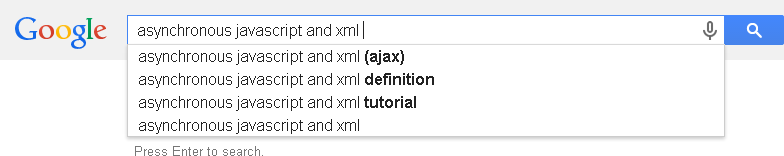
\includegraphics[scale=0.25]{../artifacts/autocomplete.png}
\caption{Autocomplete: AJAX's signature use}
\label{fig:ajax}
\end{figure}
Figure \ref{fig:ajax} only scratches the surface of AJAX. AJAX can be used to connect to databases, external APIs, and other web sites to dynamically populate a web site.
\end{frame}

\begin{frame}[fragile]
\frametitle{Simple AJAX Example}
\begin{lstlisting}[caption=Simple AJAX Example]
$(document).ready(
   function() {
      $("button").click(
         function() {
            $("#output").load("ajax.txt");
         });
   });
\end{lstlisting}
Listing 2 will populate a tag with the ID \textit{output} with the data from \texttt{ajax.txt}. The text file can act as a stand in for any external data. \cite{jquery-ajax}
\end{frame}

\begin{frame}
\frametitle{Works Cited}
\bibliography{jquery}
\end{frame}
\end{document}